\chapter{ K8051 单片机核的构建和相关设计实验}

\section{具体应用描述}

在本次实验中,我们使用 K8051 单片机核进行音乐播放器的构建和测试。

设计时设定 K8051 晶振频率为 12 MHz,依此计算延迟所需的指令周期。

实现了音乐的顺序播放与暂停功能,有瑕疵地\footnote{因此代码中不包含音乐切换的功能}完成了音乐切换的功能。

\section{Quartus下硬件设计原理图、模式及引脚说明}

\subsection{硬件设计原理图}

\begin{figure}[H]
\centering
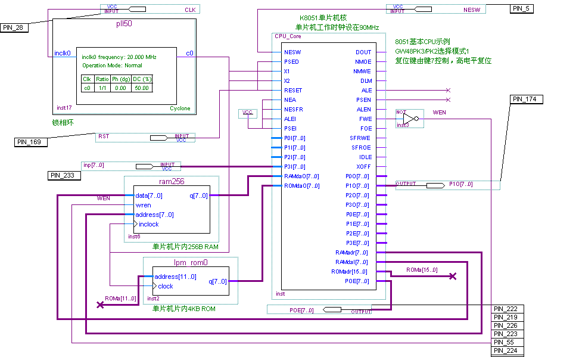
\includegraphics[width=\textwidth]{images/prin7.png}
\caption{硬件设计原理图}
\label{fig:prin7}
\end{figure}

\subsection{模式及引脚说明}

工作模式:1

\begin{table}[H]
    \centering
    \begin{tabular}{|c|c|c|}
        \hline
        描述 & 引脚 & 备注 \\
        \hline
        时钟 & 28 & CLOCK0 \\
        \hline
        复位键 & 169 & Key 7 (D15) \\
        \hline
        暂停键 & 233 & Key 1 (数码 1) \\
        \hline
        切歌键 & 237 & Key 2 (数码 2) \\
        \hline
        蜂鸣器 & 174 & SPK \\
        \hline
    \end{tabular}
    \caption{音乐播放器:引脚表}
    \label{tab:pin7}
\end{table}

\subsection{软件设计流程图及相关描述}

\begin{figure}[H]
\centering
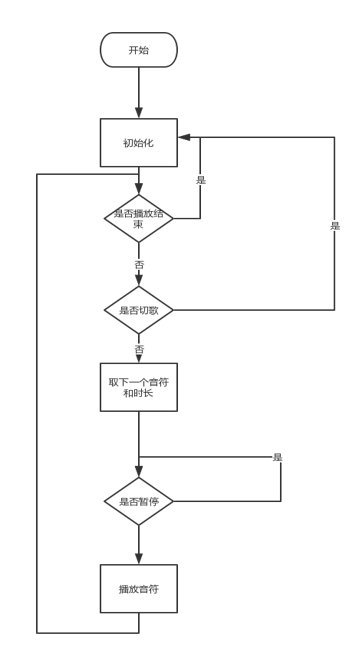
\includegraphics[width=\textwidth]{images/flow7.png}
\caption{软件设计流程图}
\label{fig:flow7}
\end{figure}

\subsection{延时计算公式}

已知 8051 晶振频率为 $F$ (Hz),每个指令需要 12 个机器周期,因此指令频率为 $\frac{F}{12}$

对于一个音符,其有频率 $f$ (Hz) 与节拍数 $p$ (单位是 1/8 节拍)。

需要事先设定一类音符的两个值:每个 1/8 拍中含有的方波个数 $s$ 与方波周期参数 $t$。

根据代码统计分析(具体见代码批注)得如下方程

$$
6 f (48 p s t + 40 p s + 36 p + 9) = p s F
$$

忽略左边的小量 $54 f$ 后可以消去 $p$ 得到

$$
24 f (12 s t + 10 s + 9) = s F
$$

再忽略左边的小量 $216 f$ 后可以消去 $s$ 得到

$$
48 f (6 t + 5) = F
$$

这样就得到了 $t$ 的近似计算公式:

\begin{equation}
t = \frac{\frac{F}{48 f} - 5}{6} \tag{1}
\end{equation}

例如对于 $F = 12,000,000$,$f = 440$,可以计算得 $t = 94$。

\section{汇编源代码}

\lstinputlisting[caption={music\_8051.asm}, label={code:music_8051}]{codes/music_8051.asm}

\section{调试总结}

调试期间出现了以下问题:

\begin{itemize}
    \item 时间紧迫,速成 8051 汇编
    
    \begin{itemize}
        \item 对指令作用理解有偏差
        \item 不恰当的代码设计模式
    \end{itemize}
    
    \item 引脚绑定错误
    
    迅速被调通。
    
    \item 程序中汇编指令逻辑错误
    
    这是常有的事情,让人充分认识到结构化程序设计里程碑式的发展。
    
\end{itemize}
